\documentclass[a4paper,12pt]{article}
%\documentclass[14pt,a4paper,twoside]{report}
\usepackage[T2A]{fontenc}
\usepackage[utf8]{inputenc}			%включаем свою кодировку: koi8-r или utf8 в UNIX, cp1251 в Windows
\usepackage[english,russian]{babel}		%используем русский и английский языки с переносами
\usepackage{amssymb,amsfonts,amsmath,mathtext,cite,enumerate,float} %подключаем нужные пакеты расширений
\usepackage[dvips]{graphicx}			%хотим вставлять в диплом рисунки?
%\usepackage{soul}
\usepackage[14pt]{extsizes}
\usepackage{longtable} 
\usepackage{graphicx}
\usepackage{indentfirst}
\usepackage{enumerate}

\graphicspath{images/}			%путь к рисункам
\bibliographystyle{unsrt}			% for bibtex

%\linespread{1.5}

\usepackage[format=plain,labelformat=simple,labelsep=endash,figurename=\CYRR\cyri\cyrs\cyru\cyrn\cyro\cyrk]{caption}
%\captionsetup{figurewithin=section}		% картинки нумеруются относительно секций
%\numberwithin{equation}{section}		% нумерация формул внутри раздела
\numberwithin{table}{section}

\makeatletter
\renewcommand{\@biblabel}[1]{#1.} 		% Заменяем библиографию с квадратных скобок на точку:
\makeatother

\RequirePackage{lscape}

\usepackage{geometry} 				% Меняем поля страницы
\geometry{left=2cm}				% левое поле
\geometry{right=1cm}				% правое поле
\geometry{top=2cm}				% верхнее поле
\geometry{bottom=2cm}				% нижнее поле

\renewcommand{\theenumi}{\arabic{enumi}}	% Меняем везде перечисления на цифра.цифра
\renewcommand{\labelenumi}{\arabic{enumi}}	% Меняем везде перечисления на цифра.цифра
\renewcommand{\theenumii}{\arabic{enumii}}	% Меняем везде перечисления на цифра.цифра
\renewcommand{\labelenumii}{\arabic{enumi}.\arabic{enumii}.}% Меняем везде перечисления на цифра.цифра
\renewcommand{\theenumiii}{\arabic{enumiii}}	% Меняем везде перечисления на цифра.цифра
\renewcommand{\labelenumiii}{\arabic{enumi}.\arabic{enumii}.\arabic{enumiii}.}% Меняем везде перечисления на цифра.цифра

\begin{document}

\title{Создание лабораторного стенда для приема сигналов спутниковых систем навигации.}
\author{Мельников А.О\\ melnikov.aleksey@gmail.com\\ МГУПИ \and Никифоров А.А.\\nikiforov.pub@gmail.com\\ МГУПИ}

\maketitle

Изучение современных беспроводных систем передачи данных предполагает проведение широкого спектра практических занятий с использованием лабораторного
оборудования.
Организация таких занятий требует значительных финансовых затрат на приобретение оборудования и поддержку его работоспособности. В этой статье мы хотели бы
рассмотреть основные подходы к организации стенда для анализа сигналов систем спутникового позиционирования.

На данный момент на рынке GNSS решений представлено 3 системы спутниковой навигации: Navstar GPS, Galileo, ГЛОНАСС. Система GPS использует методику
расширения спектра с кодированием CDMA \cite{gpsuserequipment}, в то время как Galileo и ГЛОНАСС используют частотное разделение \cite{galileo}
В данной статье мы будем оперировать
сигналом системы Navstar GPS. Поскольку он не имеет частотного разделение, в сохраненном куске данных будет содержаться информация обо всех "видных"
для приемника спутниках.
 
Мы видим три основных подхода к организации подобной лаборатории от самого дорогого, при котором используется профессиональное измерительное
оборудование с возможностью
захвата и анализа сигналов, до самого дешевого, но вместе с тем очень захватывающего, когда все придется делать своими руками.
В первом случае понадобятся: антенна GPS/GLONASS, демодулятор (downconvertor),
векторный анализатор сигналов и соединительные кабели. Основная стоимость в этом случае приходится на векторный анализатор сигналов (VSA).
Этот прибор позволяет осуществлять захват измеряемого сигнала, с возможностью его последующего анализа в оцифрованном виде.

В сценарии записи сигнала может использоваться vector signal analyzer (VSA), такой как NI PXI-5661.
Используя данную сборку, можно получить необходимый кусок "сырого" сигнала для последующей обработки.
Для каждого типа беспроводной связи требования к ширине полосы пропускания, центральной частоте и требуемое усиление разные. В
случае GPS, основным является захват 2.046МГц полосы пропускания с центральной частотой 1.57542ГГц.
Так как мощность реальнго GPS сигнала очень низка, для записи так же необходим малошумящий усилитель, такой как PXI-5690.
Так же компания поставляет набор программного обеспечения для анализа  GPS сигналов - NI GPS Toolkit для LabVIEW.
Обзор данного решения представлен в \cite{ni_vsa}.
К несомненным достоинствам решения относятся готовый набор качественного программного и аппаратного обеспечения.
Данное решение используется крупными компаниями для разработки и тестирования GPS приемников.
 
Второй подход основан на использовании стартовых или отладочных наборов для микросхем приема сигналов GNSS.
Стоимость такого набора может варьироваться от сотен долларов до нескольких тысяч.
В набор обычно входят: набор специализированного аппаратного обеспечения, иногда включается программное обеспечение.
Качество и функциональный набор ПО может варьироваться.
Данные отладочные наборы предназначены для отладки программного и аппаратного обеспечения, использующего набор
микросхем, расположенных на отладочной плате.
В качестве примера можно привести отладочную плату от компании Maxim Semiconductor на базе GPS-микросхемы MAX2769 \cite{max_evkit}.
Стоимость платы, при покупке на сайте производителя, составляет 550\$.
Программное обеспечение для данной платы позволяет перепрограммировать микросхему в разные режимы работы.
Никакого программного обеспечения обработки сигнала на сайте найти мы не смогли.

В виду высокого интереса к данной теме, некоторые университетские команды разрабатывают программное и аппаратное обеспечение
для захвата и обработки GNSS сигналов.
Как пример можно привести проект softGPS.
Ими разработано программное обеспечение демодуляции спутникового сигнала, работающее с различными front-end устройствами.
Одним из возможных вариантов для работы может являться RF front-end разработанный Денисом Акосом (Dennis Akos) \cite{akos_frontend}.
Стоимость данного устройства составляет 450\$.
Так же заслуживает отдельного внимания методология предложенная Акосом - программного приемника (software reciever).
В рамках данного подхода вся обработка сигнала ведется на программном уровне (идеальный программный приемник обрабатывает также RF тракт).
Преимуществом данного подхода является цена разработки приемника.
Обрабатывая данные на специализированных математических пакетах (Matlab, Octave), пользователь может реализовать достаточно сложные алгоритмы в примлемые
временные рамки и без финансовых вложений в разработку аппаратных решений. Это позволяет заниматься обработкой сигналов даже любителям.

Третий подход предполагает самостоятельное изготовление приемно-измерительного оборудования.
Такой подход, безусловно, является очень гибким и самым дешевым из рассматриваемых, но требует дополнительных навыков.
Так же преемуществом данного подхода является доступ к полной спецификации аппаратного обеспечения и возможнсть
разработки своего варианта программного обеспечения.
Это, безусловно, является достаточно трудоемкой задачей, но в процессе решения реализуется непосредственный
смысл разработки - создание стенда для проведения лабораторных работ.
В ходе разработки можно затронуть достаточно большое количество вопросов обработки спутникового сигнала. 

Рассмотренные нами решения позволяют оценить плюсы и минусы каждого.
К минусам VSA-устройств можно отнести высокую стоимость, но вместе с тем они обладают огромным функционалом.
При использовании отладочных наборов появляется проблема в том, что они ориентированы на прототипирование аппаратной
части и, зачастую, обладают очень скромным сопроводительным ПО.
Достаточно интересным решением может быть исходные коды проекта softGPS и аппаратная часть стороннего производителя.
Цена данного решения, относительно VSA-устройств, гораздо более привлекательна для конечного пользователя
(в отличае от крупных компаний), но все же достаточно высока.

Рассмотрев варианты, мы приняли решение разработать свой front-end модуль и ПО.
Выбрав для реализации малобюджетную GPS микросхему MAX2769 компании Maxim Semiconductor мы разработли плату под управлением ПЛИС Xilinx Spartan 2E.
Данная плата оснащена микросхемой статической памяти 256Кб.
Что позволяет сохранить чуть более 32 мс сырых данных при скорости оцифровки 16.368 Мгц.
Данного объема данных хватает для реализации лабораторной работы по обнаружению спутников.
В одной из простых реализаций параллельного алгоритма захвата сигнала от определенного спутника необходимо обрабатывать 1 мс данных.
Для более точной оценки частоты требуется 5 мс данных (алгоритм основанный на разности фаз).
Таким образом, такой конфигурации вполне достаточно для реализации поставленной задачи с минимальными
финансовыми затратами на программное и аппаратное обеспечение.
ПО управления платой, а так же VHDL код управления микросхемами на плате были реализованы нами.
Референсное ПО обнаружение спутников так же было разработано нами на Matlab/Octave с использованием подходов рассмотренных в \cite{tsui}.

Оборудование захвата представляет собой специализированный приемник сигнала GPS, позволяющий осуществить запись фрагмента сигнала от спутников.
Записанный сигнал поступает на сервер захвата и далее записывается в виде файла на публичный сервер FTP.
В текущей конфигурации \cite{gpsproject} периодически сохраняется текстовый файл flush содержащий отрезок сигнала и изображение waas\_sats с
положением спутников. Оборудование захвата содержит высокочастотный тракт, микросхему программируемой логики, память размером 256 Кбайт
для временного хранения сигнала и интерфейс RS-232 для передачи измеренного сигнала из памяти в основной сервер системы захвата.

\begin{figure}[h]
\begin{center}
    %\scalebox{0.4}{\includegraphics[width=1\linewidth]{./images/board_main.eps}}
    %\includegraphics[width=1\linewidth]{./images/board_main.eps}
\end{center}
\caption{Структурная схема платы}
\label{pic:bpsk}
\end{figure}

Сигнал спутника на частоте 1575.42МГц поступает на вход малошумящего усилителя (МШУ) и далее через ПАВ фильтр на модуль смесителя.
После смесителя выделяются две квадратурные компоненты на промежуточной частоте 4.092 МГц.
Эти сигналы поступают на двухбитовые аналого-цифровые преобразователи с частотой дискретизации 16.368 МГц.
Микропрограммное обеспечение осуществляет заполнение памяти захваченным сигналом и дальнейшую передачу этой информации
по порту RS-232 на основной сервер. Сервер осуществляет пересылку сигнала на публичный сервер ftp в виде текстового(бинарного) файла.

Рассмотрим структуру сигнала в СНС GPS. В GPS применяется фазововая схемы модуляции при кодировании информационных битов.
Фазовава манипуляция (phase shifting key - PSK).  Она была разработана  в начале развития программы исследования дальнего космоса;
сейчас схема PSK широко используется в коммерческих и военных системах связи. Фазоманипулированный сигнал имеет следующий вид \cite{sklyar}:

\begin{eqnarray}
s_i=\sqrt{\frac{2E}{T}}\cos{[{{\omega}_0}t + \phi_i(t)]}, \nonumber \\
	0\leq{t}\leq{T}, i = 1, ..., M.
\label{eq:bpsk}
\end{eqnarray}
В данном случае фазовый член ${\phi_t(t)}$ может принимать ${M}$ дискретных значений. Для случая модуляции в GPS системе ${M=2}$.
\begin{eqnarray}
	\phi_i(t)=\frac{2\pi{i}}{M}=\pi{i} \nonumber \\
	i = \{1,2\}.
\label{eq:bpsk_phi}
\end{eqnarray}
На рисунке \ref{pic:bpsk} представлена схема двочной модуляции показан переход битов 101. В формуле \ref{eq:bpsk}, ${E}$ - это энергия
сигнала, ${T}$ - время передачи символа, ${0\leq{t}\leq{T}}$. Работа схемы заключается в смещении фазы модулируемого сигнала
${s_i(t)}$ на одно из двух значений нуль(${2\pi}$) или ${\pi}$. На рисунке \ref{pic:bpsk} явно видно характерное изменение фазы при 
переходе между символами.

\begin{figure}[h]
\begin{center}
	\scalebox{0.8}{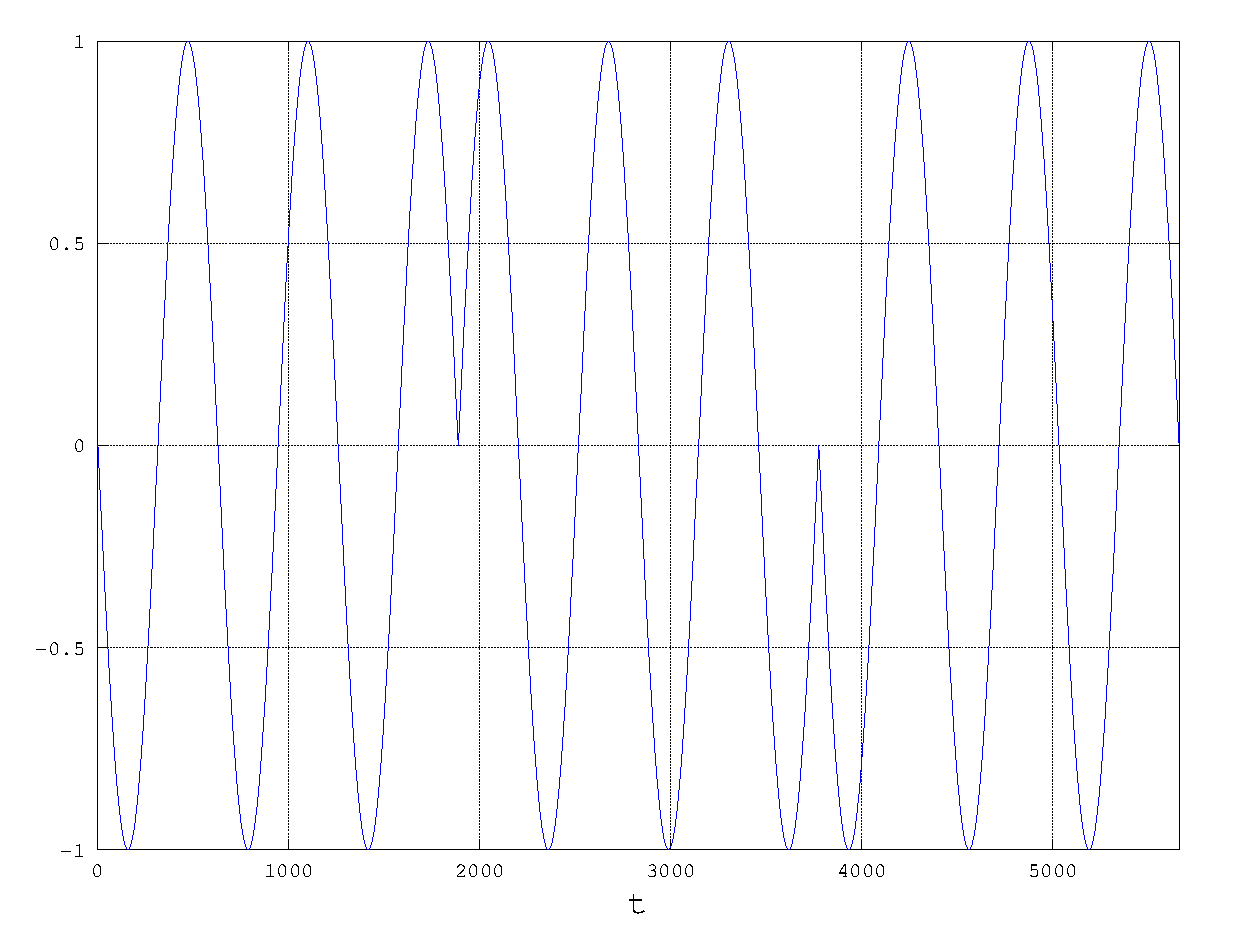
\includegraphics[width=1\linewidth]{./images/bpsk.eps}}
\end{center}
\caption{Схема модуляции BPSK}
\label{pic:bpsk}
\end{figure}

Заключение:

\bibliography{../../bibtex_db}

\end{document}
